\section{Template Method}

A ideia do Template Method é fornecer um esqueleto para um algoritmo 
e deixar para outras classes a tarefa de implementar as funções que 
compõem esse algoritmo. Uma classe abstrata define a operação Template 
Method e nela executa as etapas do algoritmo. Essas etapas são definidas 
através de operações abstratas que subclasses devem implementar para 
aproveitar o algoritmo.

Dessa forma, esse padrão ajuda a evitar repetição de código, concentrando 
em uma classe apenas a estrutura de uma operação e tornando responsabilidade 
das subclasses definir como essa operação deve ser executada. Também permite 
que um comportamento comum entre todas essas subclasses seja concentrado 
na superclasse, mais uma vez, evitando a repetição de código.

\begin{figure}[htb]
	\caption{\label{fig_grafico}Estrutura do Template Method}
	\begin{center}
	    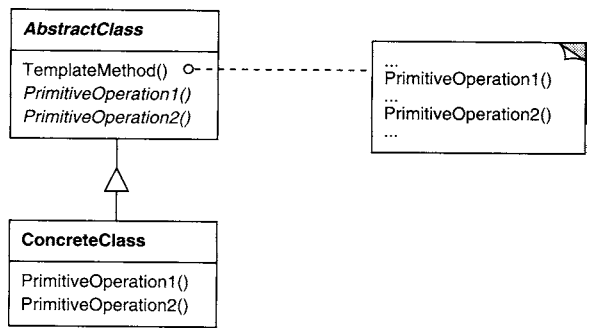
\includegraphics[scale=0.5]{5_padroes-contexto-funcional/5.3_comportamentais/5.3.10_template-method/diagram.png}
	\end{center}
\end{figure}

Exemplo Orientado a Objetos:

\begin{lstlisting}[caption={Template Method Orientação a Objetos},label=ootpmethod]
    
    abstract class AbstractClass(){
        def templateMethod() : Unit = {
            primitiveOperation1()
            predefinedOperation()
            primitiveOperation2()

        }

        def predefinedOperation() : Unit = {
            
        }

        def primitiveOperation1() : Unit

        def primitiveOperation2() : Unit
    }

    class ConcreteClass() extends AbstractClass{
        
        def primitiveOperation1() : Unit = {
            
        }

        def primitiveOperation2() : Unit = {
            
        }
    }

\end{lstlisting}

Contexto Funcional:

No contexto funcional, a mesma ideia pode ser alcançada através de 
funções de alta ordem e composição de funções. Nosso método template 
é uma função simples que recebe como parâmetro todas as funções necessárias 
para executar o algoritmo pré-definido. Caso haja alguma função comum para 
todas as possíveis versões do algoritmo, essa é simplesmente chamada dentro 
do método template como uma função comum.

Para definir uma implementação do algoritmo, basta definir uma nova função 
que é a combinação do método template com as funções que representam as 
etapas do algoritmo. Essa função executa as etapas definidas sequencialmente, 
da mesma forma que a implementação do Template Method orientado a objetos.


\begin{lstlisting}[caption={Template Method Funcional},label=fptpmethod]
    
    def predefinedOperation() : Unit =
        

    def templateMethod(primitiveOperation1 : () => Unit, primitiveOperation2 : () => Unit) = {
        primitiveOperation1()
        predefinedOperation()
        primitiveOperation2()
    }

    def primitiveOperation1() : Unit = 
        

    def primitiveOperation2() : Unit = 
        
    
    def algorithmImplementation = templateMethod(primitiveOperation1, primitiveOperation2)


\end{lstlisting}

Existe ainda uma vantagem do Template Method funcional sobre o Orientado a 
Objetos: É possível definir novos templates com operações pré-definidas 
facilmente criando uma combinação de funções que não recebe todas as 
funções do algoritmo original: [melhorar isso aqui]

Porém, uma sequência de chamadas de função se parece mais com uma 
implementação imperativa usando funções de alta ordem do que uma implementação 
funcional. Normalmente, é desejado implementar funções puras, sem efeitos 
colaterais. Para isso, seria interessante que o template method aproveitasse 
o valor de saída de uma das funções da sequência como a entrada para a 
próxima função. Isso pode ser alcançado encapsulando essa sequência de 
chamadas em um Monad:

\begin{lstlisting}[caption={Template Method Funcional: Monads},label=fptpmethodmonads]
    
    

\end{lstlisting}

É importante ressaltar que o primeiro exemplo funcional apresentado 
já implementa o Template Method. A forma como as funções são chamadas 
dentro da método template não é a parte importante do padrão, portanto 
essas funções podem ser chamadas de qualquer forma, até mesmo criando 
uma nova composição de funções. Porém, como os exemplos de Template 
Method sempre abordam a ideia de um algoritmo (sequência de passos) que 
remetem ao paradigma imperativo, é interessante mostrar que existe uma 
alternativa para essa abordagem do ponto de vista funcional também.